% % % % % % % % % % % % % %	
% %	inizio package controller

	\subsection{Romeo::Controller}
	\label{romeo::controller}
	\subsubsection{Informazioni sul package}
	\label{info_controller}
	\begin{figure}[!h]
		\centering
		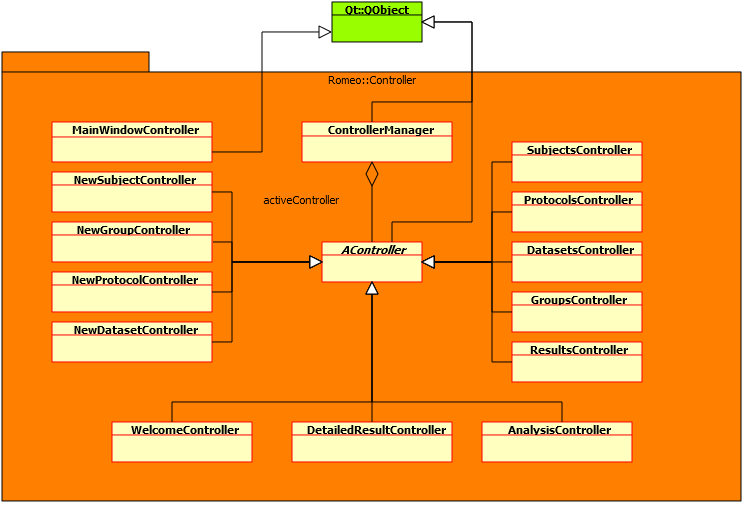
\includegraphics[width=1.1\linewidth]{./Content/Immagini/Romeo__Controller.png}
		\caption{Componente Romeo::Controller}
		\label{comp_controller}
	\end{figure}
	\subsubsection{Descrizione}
	\label{descr_controller}
	Package\glossario{} che rappresenta la componente Controller dell'architettura MVC\glossario{}.
	\subsubsection{Relazioni tra i componenti}
	La classe ControllerManager contiene dei riferimenti ai vari controller attivi.
% % % % % % % % % % % % % %		
	\subsubsection{Classi contenute}
	\paragraph{\underline{MainWindowController}}
	\label{controller_main}
		\subparagraph{Descrizione:} classe che implementa il design pattern\g{} Singleton e gestisce tutti i Signal\g{} sulle voci della toolbar.
		\subparagraph{Eredita da:}
			\begin{itemize}
				\item Qt::QObject.
			\end{itemize}
		\subparagraph{Relazioni con altre classi:}
			\begin{itemize}
				\item \hyperref[controller_wp]{Romeo::Controller::WelcomeController:} relazione entrante, la classe WelcomeController per la sua implementazione necessita di chiamare slot presenti di MainWindowController;
				\item \hyperref[mainview]{Romeo::View::Window::MainWindow:} relazione uscente, riferimento ad un oggetto MainWindow.
				\item \hyperref[nsv]{Romeo::View::Window::NewSubjectView:} relazione uscente, il controller si occupa di creare un'istanza di NewSubjectView e di aggiornare il contenuto centrale mostrato dalla MainWindow;
				\item \hyperref[controller_ns]{Romeo::Controller::NewSubjectController:} relazione uscente, il controller si occupa di creare un'istanza di NewSubjectController per controllare l'istanza di NewSubjectView precedentemente creata;
				\item \hyperref[ngv]{Romeo::View::Window::NewGroupView:} relazione uscente, il controller si occupa di creare un'istanza di NewGroupView e di aggiornare il contenuto centrale mostrato dalla MainWindow;
				\item \hyperref[controller_ngs]{Romeo::Controller::NewGroupController:} relazione uscente, il controller si occupa di creare un'istanza di NewGroupController per controllare l'istanza di NewGroupView precedentemente creata;
				\item \hyperref[npv]{Romeo::View::Window::NewProtocolView:} relazione uscente, il controller si occupa di creare un'istanza di NewProtocolView e di aggiornare il contenuto centrale mostrato dalla MainWindow;
				\item \hyperref[controller_np]{Romeo::Controller::NewProtocolController:} relazione uscente, il controller si occupa di creare un'istanza di NewProtocolController per controllare l'istanza di NewProtocolView precedentemente creata;
				\item \hyperref[ndv]{Romeo::View::Window::NewDatasetView:} relazione uscente, il controller si occupa di creare un'istanza di NewDatasetView e di aggiornare il contenuto centrale mostrato dalla MainWindow;
				\item \hyperref[controller_nd]{Romeo::Controller::NewDatasetController:} relazione uscente, il controller si occupa di creare un'istanza di NewDatasetController per controllare l'istanza di NewDatasetView precedentemente creata;
				\item \hyperref[vsv]{Romeo::View::Window::SubjectsView:} relazione uscente, il controller si occupa di creare un'istanza di SubjectsView e di aggiornare il contenuto centrale mostrato dalla MainWindow;
				\item \hyperref[controller_ss]{Romeo::Controller::SubjectsController:} relazione uscente, il controller si occupa di creare un'istanza di SubjectsController per controllare l'istanza di SubjectsView precedentemente creata;
				\item \hyperref[vgv]{Romeo::View::Window::GroupsView:} relazione uscente, il controller si occupa di creare un'istanza di GroupsView e di aggiornare il contenuto centrale mostrato dalla MainWindow;
				\item \hyperref[controller_sg]{Romeo::Controller::GroupsController:} relazione uscente, il controller si occupa di creare un'istanza di GroupsController per controllare l'istanza di GroupsView precedentemente creata;
				\item \hyperref[vpv]{Romeo::View::Window::ProtocolsView:} relazione uscente, il controller si occupa di creare un'istanza di ProtocolsView e di aggiornare il contenuto centrale mostrato dalla MainWindow;
				\item \hyperref[controller_sp]{Romeo::Controller::ProtocolsController:} relazione uscente, il controller si occupa di creare un'istanza di ProtocolsController per controllare l'istanza di ProtocolsView precedentemente creata;
				\item \hyperref[vdv]{Romeo::View::Window::DatasetsView:} relazione uscente, il controller si occupa di creare un'istanza di DatasetsView e di aggiornare il contenuto centrale mostrato dalla MainWindow;
				\item \hyperref[controller_sd]{Romeo::Controller::DatasetsController:} relazione uscente, il controller si occupa di creare un'istanza di DatasetsController per controllare l'istanza di DatasetsView precedentemente creata;
				\item \hyperref[sav]{Romeo::View::Window::AnalysisView:} relazione uscente, il controller si occupa di creare un'istanza di AnalysisView e di aggiornare il contenuto centrale mostrato dalla MainWindow;
				\item \hyperref[controller_sa]{Romeo::Controller::DatasetsController:} relazione uscente, il controller si occupa di creare un'istanza di AnalysisController per controllare l'istanza di AnalysisView precedentemente creata;
				\item \hyperref[vrv]{Romeo::View::Window::ResultsView:} relazione uscente, il controller si occupa di creare un'istanza di ResultsView e di aggiornare il contenuto centrale mostrato dalla MainWindow;
				\item \hyperref[controller_vr]{Romeo::Controller::ResultsController:} relazione uscente, il controller si occupa di creare un'istanza di ResultsController per controllare l'istanza di ResultsView precedentemente creata;
				\item \hyperref[wv]{Romeo::View::Window::WelcomeView:} relazione uscente, il controller si occupa di creare un'istanza di WelcomeView e di aggiornare il contenuto centrale mostrato dalla MainWindow;
				\item \hyperref[controller_wp]{Romeo::Controller::WelcomeController:} relazione uscente, il controller si occupa di creare un'istanza di WelcomeController per controllare l'istanza di WelcomeView precedentemente creata;
			\end{itemize}
			
	\paragraph{\underline{ControllerManager}}
	\label{controller_mn} 
		\subparagraph{Descrizione:} classe che implementa il design pattern\g{} Singleton e che contiene la lista dei controller attivi in un determinato momento. Viene utilizzata per gestire l'eliminazione di un determinato controller, attraverso il meccanismo Signal\& Slot\g{} delle Qt\glossario{}.
	\subparagraph{Eredita da:}
		\begin{itemize}
			\item Qt::QObject.
		\end{itemize}
	\subparagraph{Relazioni con altre classi:}
		\begin{itemize}
			\item \hyperref[controller_a]{Romeo::Controller::AController:} relazione uscente, riferimento all'oggetto AController attualmente presente in memoria.
		\end{itemize}
	
% % % % % % % % % % % % % %	
	\paragraph{\underline{AController}}
	\label{controller_a}
		\subparagraph{Descrizione:} classe \emph{astratta} che rappresenta un generico controller dell'applicazione \project{}.
		\subparagraph{Eredita  da:}
			\begin{itemize}
				\item Qt::QObject.
			\end{itemize}
		\subparagraph{Relazione con altre classi:}
			\begin{itemize}
				\item \hyperref[ab_panel]{Romeo::View::Window::APanel:} relazione uscente, riferimento al generico oggetto APanel che il controller sta \lq{}\lq{}controllando\rq{}\rq{}.
			\end{itemize}
		
		\subparagraph{Ereditato da:}
		\begin{itemize}
			\item \textbf{\hyperref[controller_ns]{Romeo::Controller::NewSubjectController}};
			\item \textbf{\hyperref[controller_ngs]{Romeo::Controller::NewGroupController}};
			\item \textbf{\hyperref[controller_np]{Romeo::Controller::NewProtocolController}};
			\item \textbf{\hyperref[controller_nd]{Romeo::Controller::NewDatasetController}};
			\item \textbf{\hyperref[controller_ss]{Romeo::Controller::SubjectsController}};
			\item \textbf{\hyperref[controller_sp]{Romeo::Controller::ProtocolsController}};
			\item \textbf{\hyperref[controller_sd]{Romeo::Controller::DatasetsController}};
			\item \textbf{\hyperref[controller_sg]{Romeo::Controller::GroupsController}};
			\item \textbf{\hyperref[controller_wp]{Romeo::Controller::WelcomeController}};
			\item \textbf{\hyperref[controller_sa]{Romeo::Controller::AnalysisController}};
			\item \textbf{\hyperref[controller_vr]{Romeo::Controller::ResultsController}};
			\item \textbf{\hyperref[controller_ac]{Romeo::Controller::AnalysisController}}.
		\end{itemize}
		


	\paragraph{\underline{NewSubjectController}}
	\label{controller_ns}
		\subparagraph{Descrizione:} classe che rappresenta il controller che si occupa di gestire l'interazione con l'utente durante la creazione di un nuovo Subject\glossario{}.
		Viene utilizzata per gestire i Signal\g{} emessi dalla View, riguardanti la creazione di un Subject\glossario{} e per invocare i relativi metodi del Model.
		\subparagraph{Eredita da:}
			\begin{itemize}
			 	\item \textbf{\hyperref[controller_a]{Romeo::Controller::AController}}
			 \end{itemize}
		\subparagraph{Relazioni con altre classi:}
			\begin{itemize}
				\item \hyperref[nsv]{Romeo::View::Window::NewSubjectView:} relazione uscente, tipo dinamico del riferimento ad un oggetto APanel posseduto dal controller.
			\end{itemize}
			 
	
	\paragraph{\underline{NewGroupController}}
	\label{controller_ngs}
		\subparagraph{Descrizione:} classe che rappresenta il controller che si occupa di gestire l'interazione con l'utente durante la creazione di un nuovo gruppo di Subject\glossario{}. Viene utilizzata per gestire i Signal\g{} emessi dalla View, riguardanti la creazione di un gruppo di Subject\glossario{} e per invocare i relativi metodi del Model.
		\subparagraph{Eredita da:} 
			\begin{itemize}
				\item \textbf{\hyperref[controller_a]{Romeo::Controller::AController}}
			\end{itemize}		
		\subparagraph{Relazioni con altre classi:}
			\begin{itemize}
				\item \hyperref[ngv]{Romeo::View::Window::NewGroupView:} relazione uscente, tipo dinamico del riferimento ad un oggetto APanel posseduto dal controller.
			\end{itemize}

	\paragraph{\underline{NewProtocolController}}
	\label{controller_np}
		\subparagraph{Descrizione:} classe che rappresenta il controller che si occupa di gestire l'interazione con l'utente durante la creazione di un nuovo Protocol\glossario{}. Viene utilizzata per gestire i Signal emessi dalla View, riguardanti la creazione di un Protocol\glossario{} e per invocare i relativi metodi del Model.
		\subparagraph{Eredita da:}
			\begin{itemize}
				\item \textbf{\hyperref[controller_a]{Romeo::Controller::AController}}
			\end{itemize}
		\subparagraph{Relazioni con altre classi:}
			\begin{itemize}
				\item \hyperref[npv]{Romeo::View::Window::NewProtocolView:} relazione uscente, tipo dinamico del riferimento ad un oggetto APanel posseduto dal controller.
			\end{itemize}
		
		
		
	\paragraph{\underline{NewDatasetController}}
	\label{controller_nd}
		\subparagraph{Descrizione:} classe che rappresenta il controller che si occupa di gestire l'interazione con l'utente durante la creazione di un nuovo Dataset\glossario{}. Viene utilizzata per gestire i Signal emessi dalla View, riguardanti la creazione di un nuovo Dataset\glossario{} e per invocare i relativi metodi del Model.
		\subparagraph{Eredita da:}
			\begin{itemize}
				\item \textbf{\hyperref[controller_a]{Romeo::Controller::AController}}
			\end{itemize}
		\subparagraph{Relazioni con altre classi:}
			\begin{itemize}
				\item \hyperref[ndv]{Romeo::View::Window::NewDatasetView:} relazione uscente, tipo dinamico del riferimento ad un oggetto APanel posseduto dal controller.
			\end{itemize}
		
	\paragraph{\underline{SubjectsController}}
	\label{controller_ss} 
		\subparagraph{Descrizione:} classe che rappresenta il controller che si occupa di gestire l'interazione con l'utente durante la visualizzazione dei Subject\glossario{} presenti nel sistema. Viene utilizzata per gestire i Signal\g{} emessi dalla View, riguardanti la visualizzazione dei dettagli del Subject\glossario{} selezionato, invocando i relativi metodi del Model. 
		\subparagraph{Eredita da:} 
			\begin{itemize}
				\item \textbf{\hyperref[controller_a]{Romeo::Controller::AController}}
			\end{itemize}
			\subparagraph{Relazioni con altre classi:}
				\begin{itemize}
					\item \hyperref[vsv]{Romeo::View::Window::SubjectsView:} relazione uscente, tipo dinamico del riferimento ad un oggetto APanel posseduto dal controller.
				\end{itemize}
		
		
	\paragraph{\underline{GroupsController}}
	\label{controller_sg}
		\subparagraph{Descrizione:} classe che rappresenta il controller che si occupa di gestire l'interazione con l'utente durante la visualizzazione dei gruppi di Subject\glossario{} presenti nel sistema. Viene utilizzata per gestire i Signal\g{} emessi dalla View, riguardanti la visualizzazione e la gestione dei Subject\glossario{} facenti parte del gruppo selezionato e per invocare i relativi metodi del Model. Inoltre gestirà i signal\g{} relativi alla modifica ed eliminazione dei gruppi di Subject\glossario{}.
		\subparagraph{Classi ereditate:} 
			\begin{itemize}
				\item \textbf{\hyperref[controller_a]{Romeo::Controller::AController}}
			\end{itemize}
		\subparagraph{Relazioni con altre classi:}
			\begin{itemize}
				\item \hyperref[vgv]{Romeo::View::Window::GroupsView:} relazione uscente, tipo dinamico del riferimento ad un oggetto APanel posseduto dal controller.
			\end{itemize}
		
	\paragraph{\underline{ProtocolsController}}
	\label{controller_sp}
		\subparagraph{Descrizione:} classe che rappresenta il controller che si occupa di gestire l'interazione con l'utente durante la visualizzazione dei Protocol\glossario{} presenti nel sistema. Viene utilizzata per gestire i Signal emessi dalla View, riguardanti la visualizzazione ed eliminazione dei Protocol\glossario{} facenti parte del sistema. Inoltre gestisce i signal per la visualizzazione delle informazioni sulle Feature\glossario{} ed algoritmi di clustering\glossario{} che formano il Protocol\glossario{} selezionato.
		\subparagraph{Eredita da:} 
			\begin{itemize}
				\item \textbf{\hyperref[controller_a]{Romeo::Controller::Acontroller}}
			\end{itemize}
		\subparagraph{Relazioni con altre classi:}
			\begin{itemize}
				\item \hyperref[vpv]{Romeo::View::Window::ProcolsView:} relazione uscente, tipo dinamico del riferimento ad un oggetto APanel posseduto dal controller.
			\end{itemize}
		
		
	\paragraph{\underline{DatasetsController}}
	\label{controller_sd} 
		\subparagraph{Descrizione:} classe che rappresenta il controller che si occupa di gestire l'interazione con l'utente durante la visualizzazione dei Dataset\glossario{} presenti nel sistema. Viene utilizzata per gestire i Signal emessi dalla View, riguardanti la visualizzazione ed eliminazione dei Dataset\glossario{} facenti parte del sistema. Gestisce inoltre i signal per la visualizzazione dei protocol, dei subject e informazioni aggiuntive sul dataset.
		\subparagraph{Eredita da:}
			\begin{itemize}
				\item \textbf{\hyperref[controller_a]{Romeo::Controller::AController}}
			\end{itemize}	
		\subparagraph{Relazioni con altre classi:}
			\begin{itemize}
				\item \hyperref[vdv]{Romeo::View::Window::DatasetsView:} relazione uscente, tipo dinamico del riferimento ad un oggetto APanel posseduto dal controller.
			\end{itemize}
		
		\paragraph{\underline{WelcomeController}}
		\label{controller_wp}
			\subparagraph{Descrizione:} classe che rappresenta il controller che si occupa di gestire l'interazione con l'utente durante la visualizzazione pagina iniziale. Viene utilizzata per gestire i Signal\g{} emessi dalla View, riguardanti la visualizzazione della pagina selezionata, tramite dei pulsanti presenti nella WelcomeView.
			\subparagraph{Eredita da:}
			\begin{itemize}
				\item \textbf{\hyperref[controller_a]{Romeo::Controller::AController}}
			\end{itemize}
			\subparagraph{Relazioni con altre classi:}
				\begin{itemize}
					\item \hyperref[wv]{Romeo::View::Window::WelcomeView:} relazione uscente, tipo dinamico del riferimento ad un oggetto APanel posseduto dal controller.
				\end{itemize}
		
		\paragraph{\underline{AnalysisController}}
		\label{controller_sa}
			\subparagraph{Descrizione:} classe che rappresenta il controller che si occupa di gestire l'interazione con l'utente durante l'avvio e l'esecuzione di un'analisi. Viene utilizzata per gestire i Signal\g{} emessi dalla View, riguardanti l'avvio dell'analisi e l'esecuzione dell'analisi.
			\subparagraph{Eredita da:}
			\begin{itemize}
				\item \textbf{\hyperref[controller_a]{Romeo::Controller::AController}}
			\end{itemize}
			\subparagraph{Relazioni con altre classi:}
				\begin{itemize}
					\item \hyperref[sav]{Romeo::View::Window::AnalysisView:} relazione uscente, tipo dinamico del riferimento ad un oggetto APanel posseduto dal controller;
					\item \hyperref[eav]{Romeo::View::Dialog::ExecuteAnalysisView:} relazione uscente, il controller si occupa di creare un oggetto ExecuteAnalysisView e di visualizzarlo.
				\end{itemize}
		
		\paragraph{\underline{ResultsController}}
		\label{controller_vr} 
			\subparagraph{Descrizione:} classe che rappresenta il controller che si occupa di gestire l'interazione con l'utente durante la visualizzazione della lista delle analisi effettuate e dei dettagli dei risultati di ogni analisi. Viene utilizzata per gestire i Signal emessi dalla View, riguardanti la visualizzazione dei dettagli di un'analisi, l'esportazione completa dei risultati e un'eventuale ripetizione dell'analisi. Inoltre gestisce i Signal\g{} emessi dalla View dei risultati di una particolare analisi.
			\subparagraph{Eredita da:} 
				\begin{itemize}
					\item \textbf{\hyperref[controller_a]{Romeo::Controller::AController}}
				\end{itemize}
			\subparagraph{Relazioni con altre classi:}
				\begin{itemize}
					\item \hyperref[vrv]{Romeo::View::Window::ResultsView:} relazione uscente, tipo dinamico del riferimento ad un oggetto APanel posseduto dal controller;
					\item \hyperref[drv]{Romeo::View::Window::DetailedResultView:} relazione uscente, il controller si occupa di creare un oggetto DetailedResultView e di visualizzarlo come contenuto centrale della MainWindow;
					\item \hyperref[mainview]{Romeo::View::Window::MainWindow:} relazione uscente, il controller necessità dell'oggetto MainWindow per aggiornare il contenuto da essa visualizzato.
				\end{itemize}